\documentclass[conference, onecolumn]{IEEEtran}
\IEEEoverridecommandlockouts
\usepackage{cite}
\usepackage{amsmath,amssymb,amsfonts}
\usepackage{algorithmic}
\usepackage{graphicx}
\usepackage{textcomp}
\usepackage{xcolor}
\usepackage{flushend}
\def\BibTeX{{\rm B\kern-.05em{\sc i\kern-.025em b}\kern-.08em
    T\kern-.1667em\lower.7ex\hbox{E}\kern-.125emX}}
\begin{document}

\title{SU 2024 IOT102 Bluetooth-controlled traffic light\\
}

\author{
\textsuperscript{} Pham Minh Tuan, \textsuperscript{} Hoang Trung Tin, \textsuperscript{} Huynh Quoc Khang,\\ \textsuperscript{} Nguyen Ngoc Trai, and Duc Ngoc Minh Dang\\
FPT University, Ho Chi Minh Campus, Vietnam\\
\{tuanpmse182869, tinhtse182892, khanghqse182958, trainnse182916\}@fpt.edu.vn, and ducdnm2@fe.edu.vn}
\maketitle

\begin{abstract}

Rapid urbanization and rising vehicular traffic put great pressure on traditional traffic management systems. Fixed signal timing often does not adapt to real-time traffic conditions, leading to congestion, inefficiencies, and pedestrian dissatisfaction when there are no vehicles. This article proposes a new solution: a Bluetooth-controlled traffic light system that leverages the power of Internet-of-Things (IoT) technology.\par

Our traffic light system can adjust in real-time to adjust signals quickly without the many steps of traditional traffic lights, optimizing traffic flow and minimizing delays unnecessary. Bluetooth connectivity allows authorities to intervene remotely in special situations, ensuring rapid response to traffic changes or emergencies. Additionally, the system prioritizes pedestrian safety by incorporating dedicated pedestrian crossing buttons and providing signal adjustments during low traffic times.\par

This report details the core components of the system, including the traffic light controller, Bluetooth module, and pedestrian button. We dive into the functions of each component and explain how they work together to create a responsive and adaptive traffic management solution. Furthermore, this report explores the system's potential benefits, such as reduced congestion, improved traffic flow, increased pedestrian safety and reduced emissions. We conclude by discussing the challenges associated with implementation, including concerns about security, data management, and scalability. This innovative Bluetooth-controlled traffic light system promises to revolutionize traffic management at intersections, providing a safer and more efficient traffic experience for all road users.\par

\end{abstract}

\section {\textbf{Introduction}}
The Bluetooth-controlled activity traffic light for intersection and person on foot ventures is an inventive arrangement that leverages IOT innovation to improve activity administration and improve pedestrian safety at intersections. With fast urbanization and improve pedestrian safety at intersections.With fast urbanization and increased vehicular traffic, there is an increasing demand for effective traffic management systems that can respond to changing conditions in real time.\par

So, the primary goal of our project is to design and construct a traffic light system that can dynamically modify signal timings in response to traffic circumstances.By incorporating Bluetooth connectivity, the system allows proactive remote or direct intervention of traffic light signals in special cases.\par

Bluetooth-controlled traffic light system is made up of three major components: The traffic light controller, the Bluetooth module, and the mobile application. A traffic light controller, such as using photoresistor, can be utilized as a button to assist pedestrians in changing the traffic light signal when an emergency occurs. The Bluetooth module enables wireless communication between the traffic light controller and the mobile application.\par
The mobile application has a user-friendly interface that allows authorized professionals, such as traffic operators or city officials, to remotely monitor traffic conditions and manually modify signal timings as needed.\par


In conclusion, this system, which makes use of IOT technology, has the potential to revolutionize traffic control at intersections and deliver a safer and more efficient transportation experience for both managers and pedestrians.\par


\section{Main proposal}

To develop a Bluetooth-controlled traffic light system to minimize the time spent by traffic management agencies to fine-tune the traffic lights and easily change the cycle without wasting too much time. Traditional traffic lights have disadvantages, such as being able to adjust the traffic lights, it is necessary to open the light adjustment box, and the fixed traffic light cycle during rush hour often causes congestion because the lights cannot keep up. Adjusting to the increased number of vehicles because the lights still run on a fixed cycle, pedestrians crossing the street must wait a long time at the red light even though there is no traffic. Above all, traditional traffic light control requires taking a key to open the traffic light control box, and then considering the traffic condition to control. With the above disadvantages, I would like to bring a more useful solution in optimization, the management agency only needs to stand at any location to both review the traffic situation and be able to adjust the lights easily. easier. Bluetooth traffic light systems can be easily deployed immediately, with better investment and operating costs. Smart traffic light systems controlled by Bluetooth are an effective solution for traffic regulation, helping to reduce traffic jams, guaranteeing public safety, and conserving the environment.\\


\subsection{System models and block diagram}

The created system consists of both equipment and computer programs. On the equipment side, two input types: BLUETOOTH HC05 is used to set commands to change the status of traffic light, and the Button is used to change light signals for pedestrians. Subsequently, an Arduino Uno is used as the IoT design platform, where it coordinates with the BLUETOOTH module to transfer the data to a Mobile Phone (User Phone).\par
In addition, on the programming side, a set of computer codes is written to perform the desired functions 2 (two) displays are used to show the Countdown of Traffic light(7-segment LED), and LED 8x8 displays the signal O (allowed to cross road) and X (not allowed to cross road). \par
A block diagram is presented in Fig. 1 to offer a simple way to visualize the complete system. From the block diagram, a discrete idea of all the incorporated modules/devices and their responsibilities can be achieved on a macro level.\par
\begin{figure*}[htbp]
\centerline{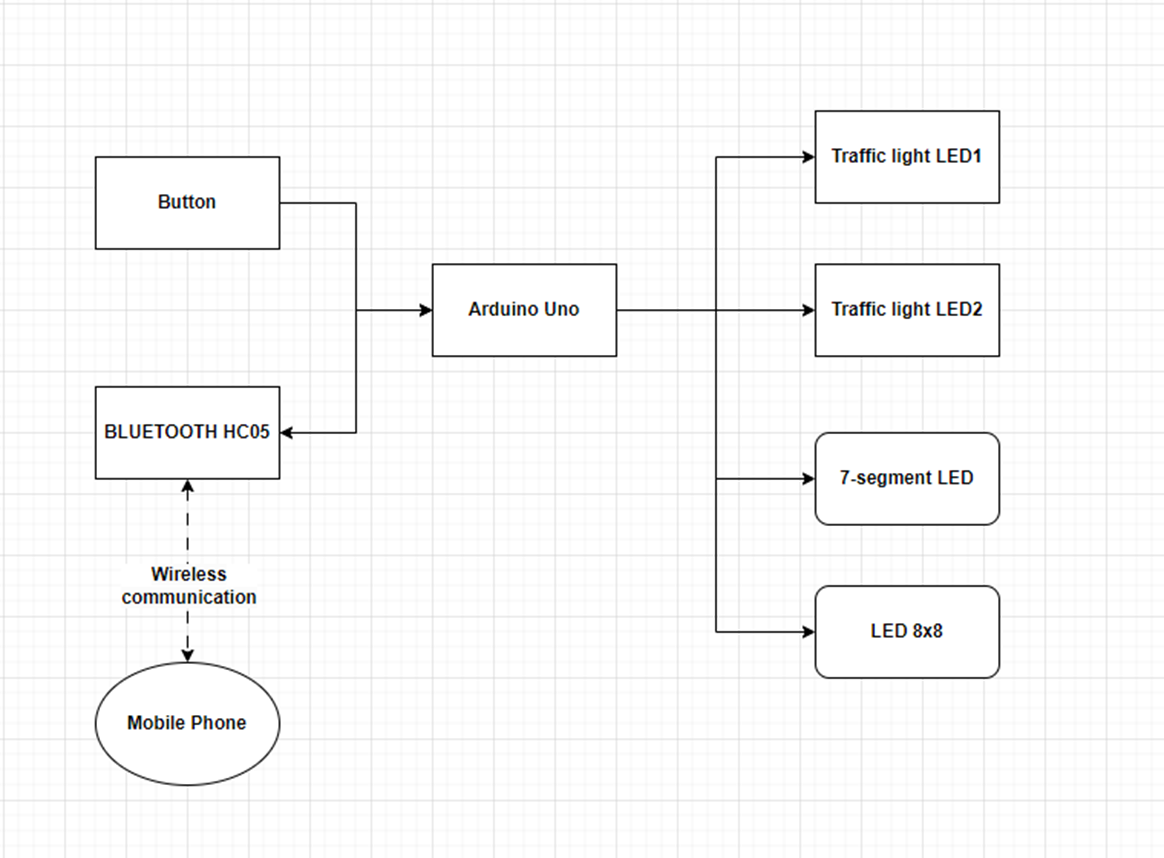
\includegraphics[width=6 in]{Block_diagram.png}}
\caption{Block diagram of the developed system.}
\label{fig}
\end{figure*}


On the input side of the Arduino Uno, there are 2 (two) inputs: BLUETOOTH HC05 and Button; and on the output side, there are 2 (two) LED control (Traffic light), 7-segment LED, and LED 8x8.\par


\subsection{Components and peripheral devices}
The Bluetooth-controlled traffic light system consists of several hardware components that work together to enable remote control and dynamic traffic management.\par

Arduino Uno Microcontroller: The Arduino Uno serves as the central processing unit of the system, responsible for interpreting commands received from the mobile app via Bluetooth and controlling the traffic light sequence.\par

The HC-05 Bluetooth Module facilitates wireless communication between the Arduino Uno and the mobile application. It establishes a Bluetooth connection and enables data exchange between the two devices.\par

Traffic Light Signal Heads: The system utilizes traffic light signal heads with red, yellow, and green LEDs to indicate the traffic flow. These signal heads receive control signals from the Arduino Uno to transition between different phases (red, yellow, green).\par

Push Button: A push button is connected to the Arduino Uno and serves as a manual override mechanism. Pressing the button allows for direct control of the traffic light sequence in case of emergencies or unexpected situations.\par

Breadboard: The breadboard provides a non-permanent and reusable platform for connecting the various electronic components of the system. It facilitates easy prototyping and experimentation without soldering or permanent connections.\par

Jumper Wires: Jumper wires are used to establish electrical connections between the Arduino Uno, Bluetooth module, push button, and traffic light signal heads. They allow for flexible and customizable wiring configurations.\par

Power Supply: A power supply delivers the necessary electrical power to the Arduino Uno, Bluetooth module, and traffic light signal heads. It ensures that the system has enough voltage and current to function properly.\par
\begin{figure*}[htbp]
\centerline{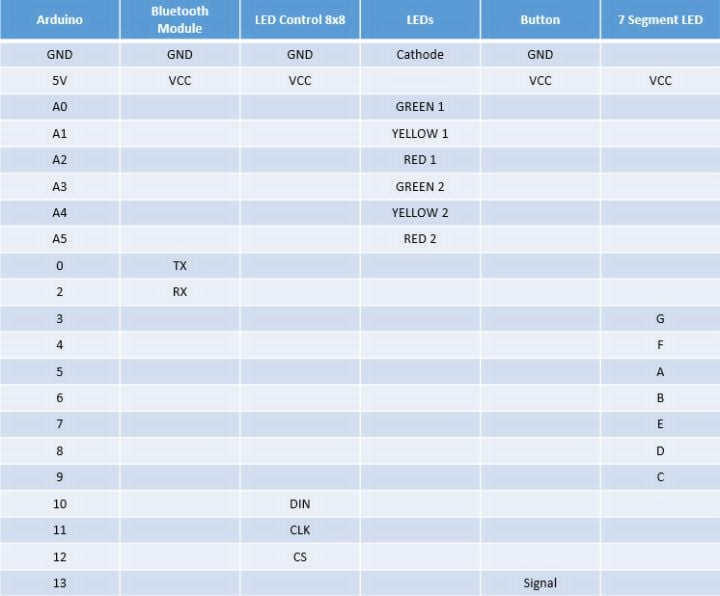
\includegraphics[width=6 in]{Table.jpg}}
\caption{Hardware interfacing of the developed system.}
\label{fig}
\end{figure*}
\subsection{Software programming}

The software programming for the Bluetooth-controlled traffic light system encompasses two main aspects:

Arduino Uno Firmware: The Arduino Uno firmware is responsible for receiving commands from the mobile app via Bluetooth, interpreting those commands, and controlling the traffic light sequence accordingly. It utilizes appropriate libraries to handle Bluetooth communication and control the GPIO pins connected to the traffic light signal heads.\par

Mobile App: The mobile app provides a user-friendly interface for interacting with the traffic light system. It allows users to select different traffic light modes (e.g., manual, timed, sensor-based), adjust timings for each phase, and monitor the current traffic flow. The program uses Bluetooth to communicate orders to the Arduino Uno so that the required traffic light control scheme can be implemented.\par

The flowchart (Figure 4) provides a visual representation of the software logic for the Arduino Uno firmware. It outlines the steps involved in receiving commands from the mobile app, interpreting those commands, and controlling the traffic light sequence.\par

The circuit (Figure 3) illustrates the hardware connections between the Arduino Uno, Bluetooth module, push button, and traffic light signal heads. It shows how the various components are interconnected to form the functional traffic light control system.\par

\begin{figure*}[htbp]
\centerline{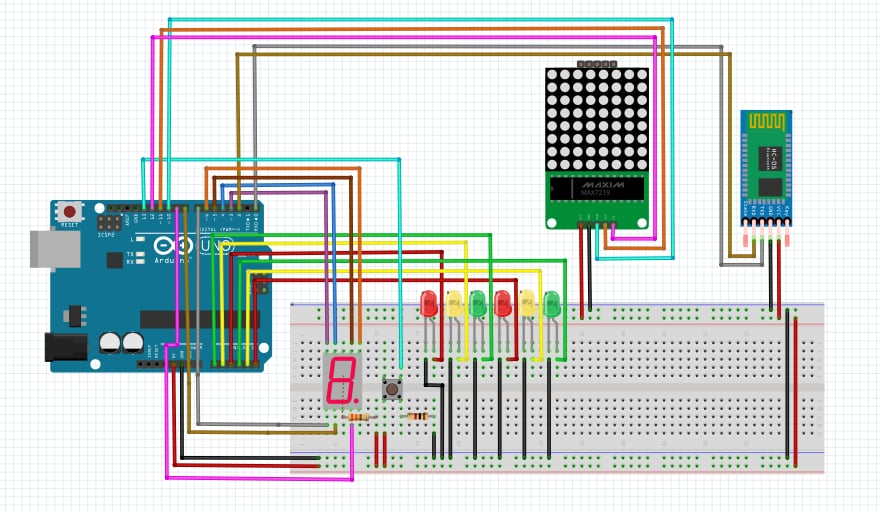
\includegraphics[width=7 in]{circuit.jpg}}
\caption{Circuit schematic of the developed system.}
\label{fig}
\end{figure*}



\section{Results and discussion}

\subsection{Prototype Implementation}
The prototype implementation of the Bluetooth-controlled traffic light system involved assembling the hardware components, connecting them according to the schematic (Figure 2), and developing the software for both the Arduino Uno and the mobile app.

1.Hardware Assembly

-Component Preparation: The required components were gathered, including the Arduino Uno, HC-05 Bluetooth module, push button, traffic light signal heads, breadboard, jumper wires, and power supply.\par

-Breadboard Setup: The breadboard was prepared by inserting power rails and connecting ground lines.\par

-Component Connections: The Arduino Uno, Bluetooth module, physical button, and traffic light signal heads were connected to the breadboard using jumper wires, following the schematic in Figure 1.\par

-Power Supply Connection: The power supply was connected to the breadboard, ensuring proper voltage and current delivery to the system.\par

2. Software Development\par

-Arduino Uno Firmware: The Arduino Uno firmware was built with the Arduino IDE. The code included libraries for Bluetooth communication and GPIO pin control. It implemented the logic for receiving commands from the mobile app, interpreting those commands, and controlling the traffic light sequence appropriately.\par

-Mobile App Development: The mobile app was developed using a suitable programming language and development environment. It provided a user interface for selecting traffic light modes, adjusting timings, and monitoring traffic flow. The app communicated with the Arduino Uno via Bluetooth to send control commands.\par

3.Testing and Evaluation\par

-Initial Testing: The prototype was initially tested for basic functionality, ensuring proper communication between the Arduino Uno and the mobile app. The traffic light sequence was manually controlled from the app to verify that the system responded correctly to commands.\par

-Mode Testing: Different traffic light modes (e.g., manual, timed, sensor-based) were tested to ensure that the system could transition between modes and operate as expected in each mode.\par

-Timing Adjustments: The timing of each traffic light phase (red, yellow, green) was adjusted and tested to ensure that the system could effectively manage traffic flow.\par

-Error Handling: The system was tested for potential errors and unexpected scenarios, such as loss of Bluetooth connection or power interruptions.\par


\subsection{Programming Flowchart}
The flowchart in Fig.4 depicts how our Bluetooth traffic light system works

\begin{figure*}[htbp]
\centerline{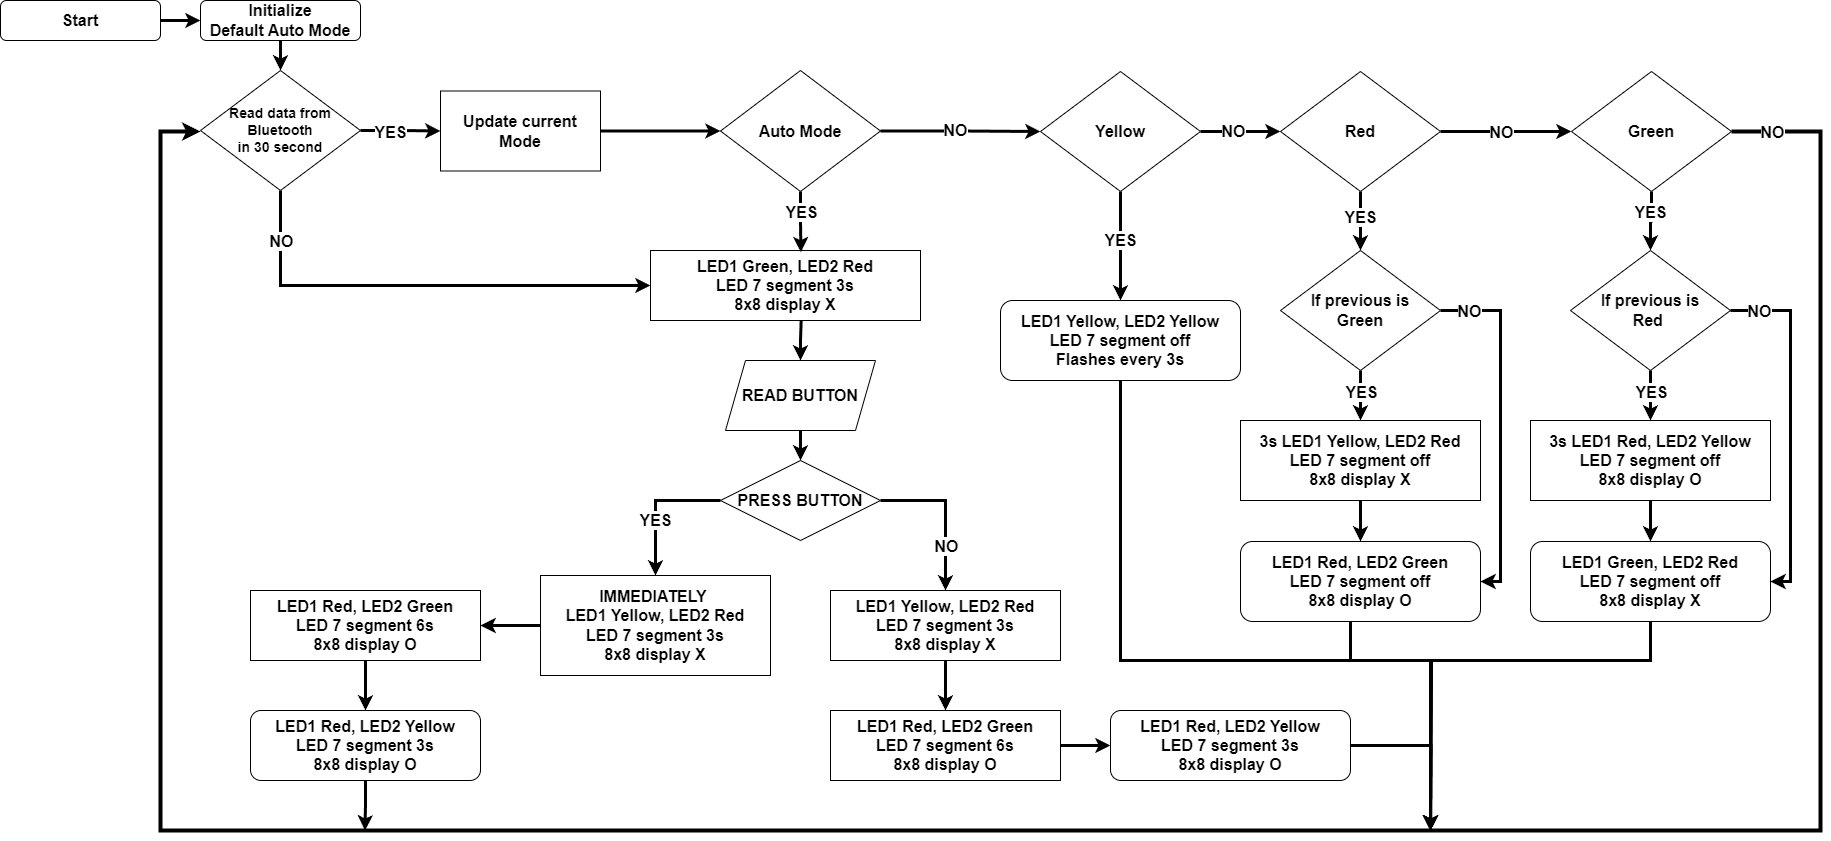
\includegraphics[width=7 in]{FlowChart-final_1.drawio.png}}
\caption{Flowchart diagram of the developed system.}
\label{fig}
\end{figure*}



\subsection{Experimental Results}
To ensure convenience for traffic polices, the Arduino system will automatically enter auto mode upon startup. In auto mode, traffic light column 1 will turn green for 3 seconds, indicating that traffic on the straight road is allowed to proceed. Concurrently, the 7-segment LED will display a countdown timer corresponding to the green light duration, and the 8x8 LED Matrix will show an 'X' to indicate that pedestrians are not allowed to cross during this period. Meanwhile, traffic light column 2 will display red to signal that traffic on the intersecting road must stop.\par

When the countdown hits zero, traffic light column 1 will turn yellow for 3 seconds to signal to vehicles on the straight road to slow down and prepare to stop at the line, letting cars from the next road pass. During this period, the 7-segment LED continues to count down, the 8x8 LED Matrix will still show an 'X', and traffic light column 2 will remain red.\par

After the yellow light countdown ends, traffic light no.1 will turn red signal for 6 seconds, indicating that vehicles on the straight road must come to a complete stop to yield to the intersecting road traffic. The 7-segment LED will display the countdown, the 8x8 LED Matrix will show an 'O' to signal that pedestrians are now allowed to cross, and traffic light column 2 will turn green for 3 seconds to allow traffic on the intersecting road to move. If the countdown reaches 3 seconds, traffic light column 2 will turn yellow, signaling drivers to slow down and yield to the traffic on the straight road. When the countdown ends, traffic light column 1 will turn green again for 3 seconds, resuming the cycle. During this phase, the 7-segment LED will display the countdown, the 8x8 LED Matrix will show an 'X', and traffic light column 2 will turn red to stop intersecting road traffic.\par

A button feature has been added to improve pedestrian convenience. If a pedestrian want to cross while traffic signal column 1 is green, they can press the button. Upon pressing, traffic light column 1 will switch to yellow for 3 seconds, then turn red for 6 seconds, allowing the pedestrian to cross safely. The 7-segment LED will display the countdown, the 8x8 LED Matrix will show an 'O' to signal pedestrian crossing, and traffic light column 2 will turn green, allowing traffic on the intersecting road to move.\par

If a phone sends Bluetooth data with the characters "R", "Y", "G", or "A", auto mode will be interrupted and switch to the corresponding manual function. As auto mode is disabled, the 7-segment LED will be turned off as well. If the Arduino receives the character "R" from Bluetooth, traffic light column 1 will turn red to signal that traffic on the straight road must stop, the 8x8 LED Matrix will display 'O' allowing pedestrian crossing, and traffic light column 2 will turn green to allow traffic on the intersecting road to proceed.\par

If the Arduino receives the letter "G", traffic light column 1 will change green, allowing traffic on the straight road to proceed, the 8x8 LED Matrix will display 'X' denying pedestrian crossing, and traffic light column 2 will turn red, stopping traffic on the intersecting road.\par

To guarantee the safety of all road users, if the system changes from "R" to "G" or vice versa, both traffic lights will not change immediately as expected. Instead, traffic light column 1 will remain red for an additional 3 seconds, and traffic light column 2 will switch to yellow for 3 seconds to signal that traffic on the intersecting road should slow down and stop at the line. After these 3 seconds, traffic light column 1 will turn green, and traffic light column 2 will turn red.\par

If the Arduino receives the character "Y", both traffic lights will glow yellow and change every 3 seconds. The flashing yellow light warns cars to continue with caution, lower speed, examine their surroundings, and yield to pedestrians. This process will continue until a new command is entered.\par

A safety mechanism is developed to prevent traffic enforcers from disconnecting Bluetooth and forgetting to restart auto mode after a previous "R" or "G" order. If no Bluetooth data is received within 30 seconds, the system will automatically revert to auto mode, and the 7-segment LED will resume the countdown. Traffic enforcers can also input the command "A" to rapidly return to auto mode if necessary. See more in Fig.4 \par

\subsection{Discussion}
The Bluetooth-controlled traffic light system described in this research is a viable method for improving traffic management and pedestrian safety at intersections. The system uses Internet of Things (IoT) technology to enable lights to dynamically adjust in reaction to current traffic conditions, thereby minimizing congestion and enhancing overall traffic flow. Furthermore, Bluetooth connectivity allows for remote or direct direct action in emergency situations or during periods of high pedestrian density.\par

The effectiveness of the Bluetooth control system is demonstrated by its ability to reduce traffic congestion and management agencies can easily make changes without too many steps. By altering flag timing based on real-time activity information, the framework can minimize pointless delays and optimize the activity stream, particularly amid surge hours. This can save significant time for both drivers and pedestrians while also reducing fuel usage and emissions while waiting at red lights.\par

Furthermore, the Bluetooth control system improves pedestrian safety by incorporating a pedestrian button and providing pedestrian-specific signal phases. This feature allows pedestrians to safely cross intersections even when vehicle density is minimal, ensuring their safety and improving overall traffic safety.\par

Compared to traditional time-based traffic lights, Bluetooth-controlled systems offer several advantages. Traditional traffic lights use a fixed signal cycle, which may not be optimal for varying traffic conditions from time to time. This can lead to congestion during rush hour and delays for pedestrians during low traffic times. On the other hand, the Bluetooth control system can flexibly adjust signal timing to suit the current traffic situation, allowing traffic to be distributed more effectively and improving safety for all traffic participants.\par

Besides the potential benefits, Bluetooth control systems also pose some challenges that need to be addressed for successful implementation. One concern is the security of the Bluetooth connection as unauthorized access could affect the system's operation and the distance to be able to use Bluetooth is within 10 meters. Strong security mechanisms, such as encryption and authentication procedures, should be established to prevent unwanted access and protect system integrity while in use, but speed must also be maintained.

\begin{table}[htbp]

\begin{center}


\begin{tabular}{|c|l|l|c|}
\hline
\textbf{No}&\textbf{Task} & \textbf{Result form}& \textbf{Time schedule} \\
\hline
1 & Writing proposal & Proposal & May 20-27, 2024 \\
\hline
2 & Understand Traditional Traffic Light Operation &Simulation diagram (.png) & May 24-26, 2024 \\
\hline
3 & Draw Simulation Diagram &Simulate using bluetooth & May 25, 2024 \\
\hline
4 & Component Selection &Component  & May 30-June 7, 2024 \\
\hline
5 & Draw Block Diagram &design details & June 9, 2024 \\
\hline
6 & Draw Flowchart &software logic & May 30-June 15, 2024 \\
\hline
7 & Write Code &Fix bugs and test run & May 30-June 30, 2024 \\
\hline
8 & Test &check logic & June 15-June 30, 2024 \\
\hline

9 & Writing final paper & Paper & Jun 1-7, 2023 \\
\hline
\end{tabular}
\label{tab1}
\end{center}
\end{table}

\section{Conclusion}
In conclusion, the Bluetooth-controlled traffic light project offers several advantages in terms of flexibility, energy efficiency, smart management, and ease of installation and scalability. By enabling remote control of traffic signals through Bluetooth connectivity, the project allows for dynamic control of traffic flow, making it useful in densely populated areas, special events, or emergency situations.\par

The system can be designed to automatically adjust traffic signals based on real-time data and other parameters, reducing waiting times and saving energy by activating lights only when necessary. Besides, the collected information from the traffic lights can be utilized for traffic investigation, design recognizable proof, and traffic flow optimization, driving to progressed traffic efficiency and blockage less. The utilization of Bluetooth network simplifies the establishment preparation and encourages framework.\\

\section{Reference to Future work}
While this research has demonstrated the feasibility of a Bluetooth-controlled traffic light system, it is essential to acknowledge that there are areas for improvement. One critical challenge lies in enhancing the system's security to mitigate risks such as unauthorized access and data breaches. Additionally, the limitations of Bluetooth connectivity, particularly in terms of range, interference, and weather require further investigation.\par

It is essential to gather and examine past traffic signal data to maximize traffic flow and spot possible bottlenecks. These data, including cycle times and usage patterns, can be stored in a dedicated database for in-depth analysis. By leveraging this information, traffic management agencies can make data-driven decisions to improve traffic efficiency.\par

Developing a user-friendly mobile app to control and monitor traffic lights remotely is another promising avenue for future research. The app could provide real-time traffic updates, allow users to adjust traffic light timings, and potentially offer historical traffic data visualization. Cross-platform development frameworks like Flutter or React Native can be utilized to ensure compatibility across different mobile devices.\par

By addressing these areas, future research can contribute to developing more robust, efficient, and user-centric Bluetooth-controlled traffic light systems.\\


\section{Author's contribution}
    

\begin{table}[h!]
\centering
\caption{Author's contribution}
\label{tab:my_label}
\begin{tabular}{|c|c|c|c|c|}
\hline
\#& Student ID & Student Name & Tasks & Contribution\\
\hline
1& SE182958& Huynh Quoc Khang& Draw block diagram, flowchart& 25\%\\
\hline
2& SE182869& Pham Minh Tuan& Study conception and design& 25\%\\
\hline
3& SE182916& Nguyen Ngoc Trai& Program Arduino and BLUETOOTH HC05& 25\%\\
\hline
4& SE182892& Hoang Trung Tin& Write report, prepare Presentation& 25\%\\
\hline
\multicolumn{4}{|c|}{Total}& 100\%\\
\hline
\end{tabular}
\end{table}


\end{document}
